\documentclass[tikz,border=10pt]{standalone}
\usepackage{tikz}
\usetikzlibrary{angles,quotes,calc}
\usepackage{tkz-euclide} %for right angle marker

\begin{document}
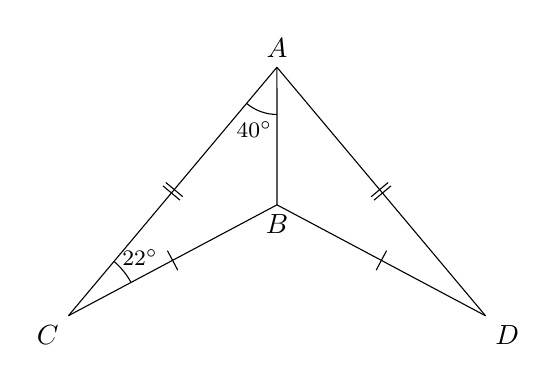
\begin{tikzpicture}[scale = 1.5]
    % Initial point
    \coordinate (C) at (0,0);
    % Draw base
    \draw (C) -- ++(28:2cm) coordinate (B);
    
    % % Draw triangle
    \path[name path=leg1] (B) -- ++(90:1.5cm);
    \path[name path=leg2] (C) -- ($(C)!1.5!22:(B)$) coordinate (L);
   
    \draw[name intersections={of=leg1 and leg2,by={A}}] (B) -- (A);
    \draw (C) -- (A);

     % Draw triangle 2
    \path[name path=leg3] (A) -- ($(A)!2.5!40:(B)$);
    \path[name path=leg4] (B) -- ($(B)!1!124:(C)$) ;
    \draw[name intersections={of=leg3 and leg4,by={D}}] (D) -- (A);
    \draw (D) -- (B);

    % Label points E and B
    \node at (A) [anchor=south] {$A$};
    \node at (B) [anchor= north] {$B$};
    \node at (D) [anchor = north west] {$D$};
    \node at (C) [anchor = north east] {$C$};

    \tkzMarkSegment[pos=.5,mark=||](A,C);
    \tkzMarkSegment[pos=.5,mark=||](A,D);
    \tkzMarkSegment[pos=.5,mark=|](C,B);
    \tkzMarkSegment[pos=.5,mark=|](D,B);
    
    % % Draw the angle between lines
    \pic [draw, "\footnotesize $40^\circ$ ", angle eccentricity=1.4, angle radius=0.6cm] {angle = C--A--B};
    \pic [draw, "\footnotesize $22^\circ$", angle eccentricity=1.3, angle radius=0.9cm] {angle = B--C--A};
   
\end{tikzpicture}
\end{document}

